\documentclass[10pt]{beamer}

\usetheme[progressbar=frametitle]{metropolis}

\usepackage{booktabs}
\usepackage[scale=2]{ccicons}

\usepackage{pgfplots}
\usepgfplotslibrary{dateplot}

\usepackage{xspace}
\newcommand{\themename}{\textbf{\textsc{Rendezvous}}\xspace}

% my configuration 
\usepackage{ragged2e} % for alignment of paragraph
% my configuration
\usepackage[font=small,skip=0pt]{caption} % spacing between figure and image
% my configuration for indicator  (math)
\usepackage{dsfont}
% my configuration: reduce spacing between text and equation
\expandafter\def\expandafter\normalsize\expandafter{%
    \normalsize
    \setlength\abovedisplayskip{0pt}
    \setlength\belowdisplayskip{0pt}
    \setlength\abovedisplayshortskip{0pt}
    \setlength\belowdisplayshortskip{0pt}
}
\newcommand*{\perm}[2]{{}^{#1}\!P_{#2}}%
\newcommand*{\comb}[2]{{}^{#1}C_{#2}}%

\title{Power Save on 802.11ax MAC}
%\subtitle{}
\date{\today}
\author{Yang Hang \\ Advisor: K.C. Chen}
\institute{Gratitude Institute of Communication Engineering }
\titlegraphic{\hfill
\includegraphics[height=1.5cm]{logo}}

\begin{document}

\maketitle
% frame
\begin{frame}{Table of contents}
	\setbeamertemplate{section in toc}[sections numbered]
    \setbeamertemplate{subsection in toc}[subsections numbered]
    % my configuration
\setcounter{tocdepth}{5}
\setcounter{secnumdepth}{5} 
    \tableofcontents%[hideallsubsections]
\end{frame}

\section{802.11 MAC and its Power Save}
% frame
\begin{frame}{802.11 MAC--DCF}
Before 802.11ac, wifi use a single-user \alert{(SU) PHY}, i.e., only one node could access at a time. \\
Distributed Coordination Function (DCF) is a random access mechanism. 
All nodes including stations (STAs) and access point (AP) need contend to access the channel. \\
DCF is a simple and flexible mechanism so that it works on unlicensed band. 
\begin{figure}
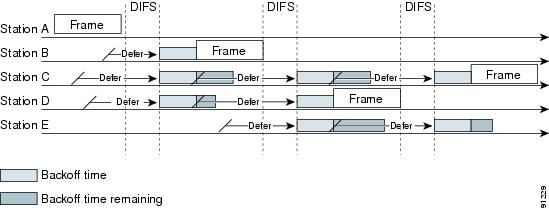
\includegraphics[scale=0.6]{./figure/DCF.jpg}
\caption{DCF example}
\end{figure}
\end{frame}

% frame
\begin{frame}{Energy Consumption of WiFi}
Since most AP is powered with wire, energy consumption of STAs deserves our concern.
Several sources of energy waste of a STA are as follows \cite{ye2002energy}.
\begin{enumerate}
\item \textbf{Idle Monitoring} 
\item \textbf{Collision} It is serious in dense network.
\item \textbf{Overhearing} 
\item \textbf{Control Packet Overhead} Like RTS/CTS, ACK.
\item \textbf{Header Overhead} It is necessary for an unscheduled mechanism.  
\end{enumerate}
Actually, all the up-link (UL) transmission is effective, since STAs know UL arrival time once UL packet arrives.
Unfortunately, STAs don't know when down-link (DL) packets come.
They need \alert{stay active all the time} to get ready for a DL transmission intuitively. 
\end{frame}

% frame 
\begin{frame}{Working State Occupation\cite{lin2005comprehensive}}
\begin{figure}
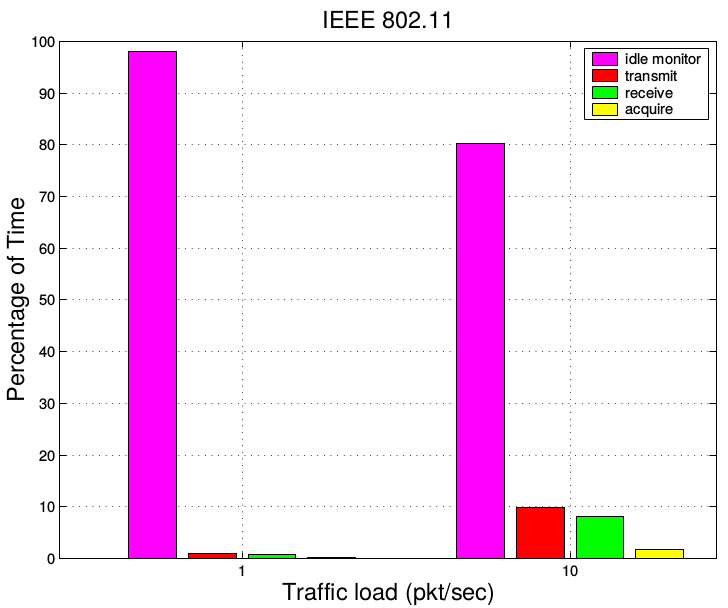
\includegraphics[scale=0.35]{./figure/energy_consumption.png}
\caption{A Node's Dwell Time in Different States}
\label{fig_workoccupation}
\end{figure}
\end{frame}

% frame
\begin{frame}{Power Save Mode (PSM) of legacy WiFi}
See a successful transmission as a rendezvous between AP and STA. 
Three classes of Rendezvous Schemes:
\begin{itemize}
\item Synchronous Scheme
\item Pseudo-synchronous Scheme, cycled receiver
\item Asynchronous Scheme, wakeup radio
\end{itemize}
Since UL transmission is effective transmission, legacy PSM, called \alert{Periodical Listen and Sleep}, only concerns about DL transmission. It belongs to \textbf{Pseudo-synchronous Scheme}. 
\end{frame}

% frame
\begin{frame}{Legacy PSM: Periodical Listen and Sleep}
\textbf{Key components:} Beacon and Traffic Indicate Map (TIM), listen interval, PS-poll packet.   
\begin{figure}
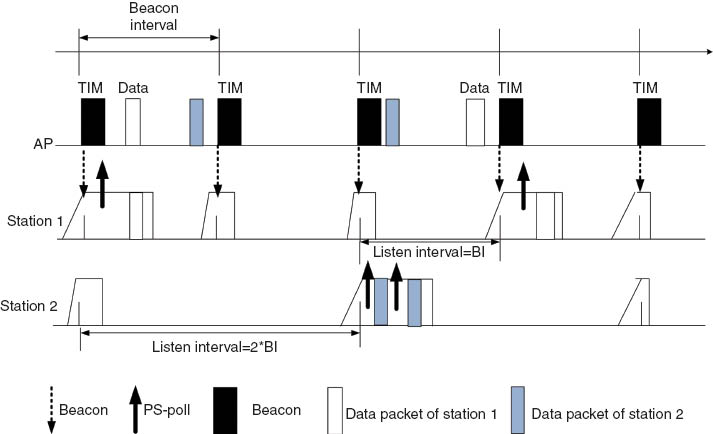
\includegraphics[scale=0.8]{./figure/legacy_PSM.jpg}
\label{legacy_PSM}
\end{figure}
\end{frame}

\section{Difference in 802.11ax MAC}
% frame
\begin{frame}{Key Features of 802.11ax MAC}
OFDMA helps realize \alert{MU PHY} in 802.11ax, as a result leading to Trigger-based UL. See figure \ref{fig_mu_ul}.\\
DCF doesn't care about UL/DL fairness. Legacy AP is almost equal to STAs on MAC. However, the star topology determines the priority status of AP in BSS. In 802.11ax, UL and DL are both scheduled by AP. \textbf{An efficient scheduler} is needed. 
% also interference may destroy the design. Think about that.
Here, we focus on the \textbf{energy efficiency}.\\
Proposed PSMs for 802.11ax are as following slides. 
\begin{figure}
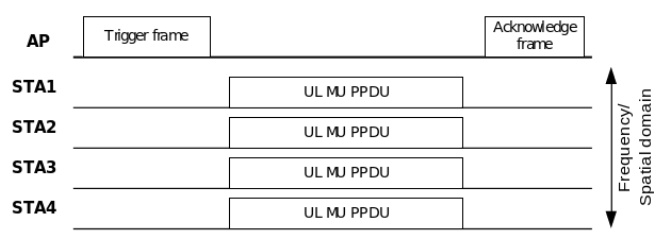
\includegraphics[scale=0.35]{./figure/mu_ul.png}
\caption{trigger-based MU UL\cite{mu_ul}}
\label{fig_mu_ul}
\end{figure}
\end{frame}

% frame
\begin{frame}{Passive PS (PPS)}
Passive PS save power by turning off its radio until the end of transmission of intra-BSS for others.  
To realize this mechanism, \textbf{BSS color}, \textbf{STA identifier}, \textbf{UL/DL indicator} are set in HE-SIG-A/HE-SIG-B.

According to \cite{pps}, an HE STA may enter the Doze state until the end of an PPDU if the following conditions are true:
\begin{itemize}
\item
same BSS color
\item 
DL but not the same identifier; or UL
\end{itemize}
\begin{figure}
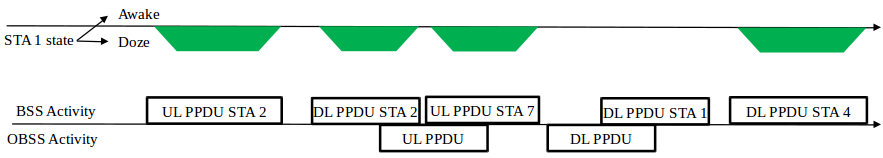
\includegraphics[scale=0.3]{./figure/pps.png}
\caption{Passive PS for 802.11ax\cite{pps}}
\label{pps}
\end{figure}
\end{frame}

% frame
\begin{frame}{PS for Random Access (PSRA)}
Since trigger frame for random access (TF-R) proceeds the UL transmission, STA couldn't start UL transmission until TF-R arrives. 
STA could "sleep" until TF arrives. That's the intuitive idea behind PSRA. 
\begin{figure}
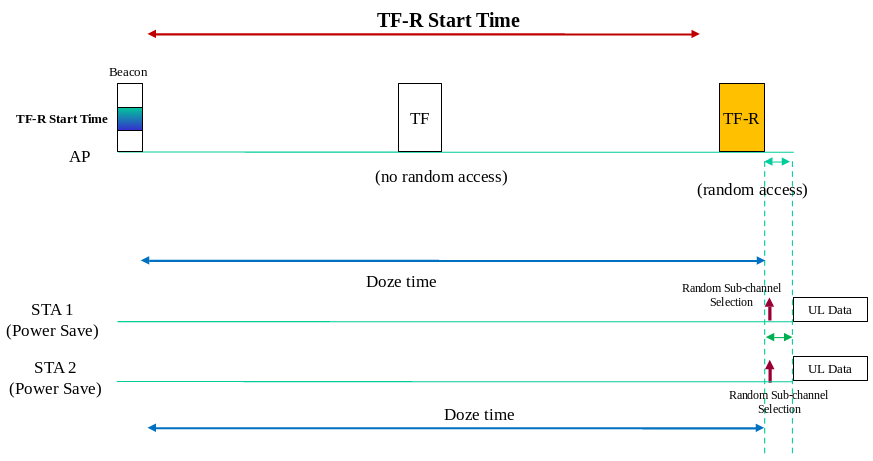
\includegraphics[scale=0.34]{./figure/psra.png}
\caption{PSRA\cite{psra}}
\label{psra}
\end{figure}
\end{frame}

% frame
\begin{frame}{Problems of Proposed PSM for 802.11ax}
\begin{itemize}
\item
PPS helps PS by reducing the waste energy on \textbf{overhearing}. The heavier loading traffic, the more energy are saved. 
However, it doesn't help for \textbf{idle monitoring}, see Figure \ref{fig_workoccupation}. 
Thus, it works as an\textbf{•} auxiliary PSM. 
\item
Current PSRA is \textbf{not} a complete approach. 
\end{itemize}
Since before 802.11ax, UL is scheduled by STAs themselves. 
Legacy PSM has been well designed for DL traffic, which still works on 802.11ax. 
While trigger-based UL is the main difference from legacy 802.11 versions, we will \textbf{focus on PS for UL}.
\end{frame}

\section{My PS design for 802.11ax UL}
\subsection{Design Description}
% frame
\begin{frame}{My PS design for 802.11ax UL}
    Since UL is based on triggered frame (\textbf{TF}), design as follows:
    \begin{enumerate}
    \item
    Two kinds of TF are issued here. \textbf{TF-R} for request collection, regular \textbf{TF} for resource allocation.
    \item
    TF-R is scheduled periodically with well-known period $T$.
    \item
    Resource Request (\textbf{RR}) procedure includes contending and selection. 
    When number of success contending STAs is large, AP has not enough resource to allocate, then selecting some to allocate resource. 
    \item
    \textbf{More bit} is set when the allocated resource is not enough for the UL traffic.  
	%A maximum duration for UL is denoted by $T_u$.
    \end{enumerate}
	    
    \begin{figure}
    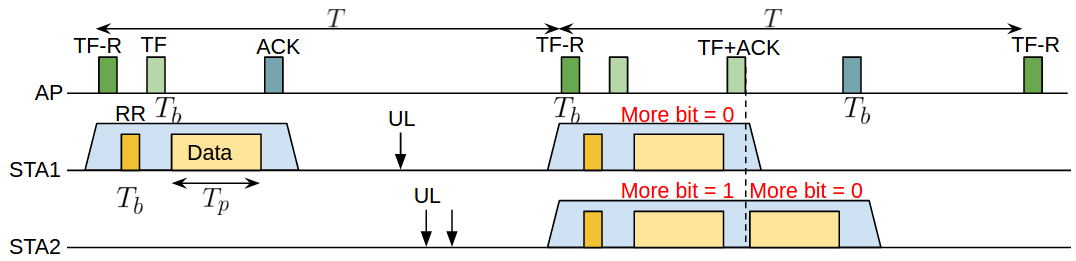
\includegraphics[scale=0.25]{./figure/ps_ax.png}
    \caption{PS for 802.11ax UL}
    \label{ps_ax}
    \end{figure}
\end{frame}

\subsection{Problem Formulation}
% frame
\begin{frame}{Problem Formulation}
	\metroset{block=fill}
	\begin{block}{Assumption}
	\begin{itemize}
		\item 
		No channel fading
		\item
		$P_{TX}$ is a constant
		\item
		Assume random access for RR with constant contention window
		\item
		IFS and TF-R's DCF contending is ignored.
		\item
		Poisson Arrival $\lambda$ for each STA UL
	\end{itemize}    
    \end{block}
 % equation
\begin{equation}
\label{equ_energy}
E = \bigtriangleup_{RX}P_{TX} + \bigtriangleup_{TX}P_{RX} + \bigtriangleup_{idle}P_{idle} + \bigtriangleup_{doze}P_{doze} 
\end{equation}

We only consider UL traffic here. 
Since IFS and DCF contending are ignored here and STAs know when TF-R will arrive, 
with PS, STA could wake up only for transmission. That means no idle state. 
On the contrary, without PS, duration of doze state is replaced by idle state. 
\begin{align}
\label{equ_idle}
\text{with PS}	 &: \; \bigtriangleup_{doze} = 1 - \bigtriangleup_{RX} - \bigtriangleup_{TX} \\
\label{equ_doze}
\text{without PS} &:\; \bigtriangleup_{idle} = 1 - \bigtriangleup_{RX} - \bigtriangleup_{TX} 
\end{align}
\end{frame}

% frame
\begin{frame}{$\bigtriangleup_{TX}$ and $\bigtriangleup_{RX}$ Representation}
\metroset{block=fill}
\begin{alertblock}{Notations}
	$D^s_{TX}$: Duration of TX in successful Resource Request (\textbf{RR})\\ 
	$D^f_{TX}$: Duration of TX in failing \textbf{RR} \\
    $p_s$: prob. of suc \textbf{RR} \\
    $p_t$: transmit prob. of STA
\end{alertblock}
All variables following should be expected value.
% equation
\begin{equation}
\label{equ_tx}
\bigtriangleup_{TX} = \frac{1}{T}[D_{TX}^sp_s + D_{TX}^f (1-p_s)]p_t
\end{equation}
% equation 
\begin{equation}
\label{equ_rx}
\bigtriangleup_{RX} = \frac{1}{T}[D_{RX}^sp_s + D_{RX}^f (1-p_s)]p_t
\end{equation}
% figure
\begin{figure}
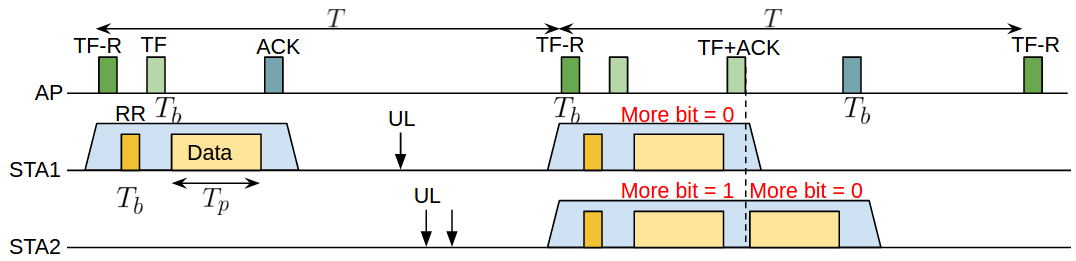
\includegraphics[scale=0.25]{./figure/ps_ax.png}
\label{fig_ps_ax_2}
\end{figure}
\end{frame}

% frame
\begin{frame}{$D_{TX}^s$,$D_{TX}^f$,$D_{RX}^s$,$D_{RX}^f$}
% block
\metroset{block=fill}
\begin{alertblock}{Notations}
    $T_b$: time for transmitting a control frame \\
	$T_p$: time for transmitting a data frame under normal data rate\\
	$UL$: num. of UL packets to be sent in current TF period given suc RR\\        
    $R$: allocated resource  (normalized date rate)
\end{alertblock}
\begin{align}
D_{TX}^s = \frac{UL}{R}T_p + T_b,\quad
 &D_{TX}^f = T_b \\
D_{RX}^s =  (UL + 2)T_b,\quad
 & D_{RX}^f = 2T_b
\end{align}
% figure
\begin{figure}
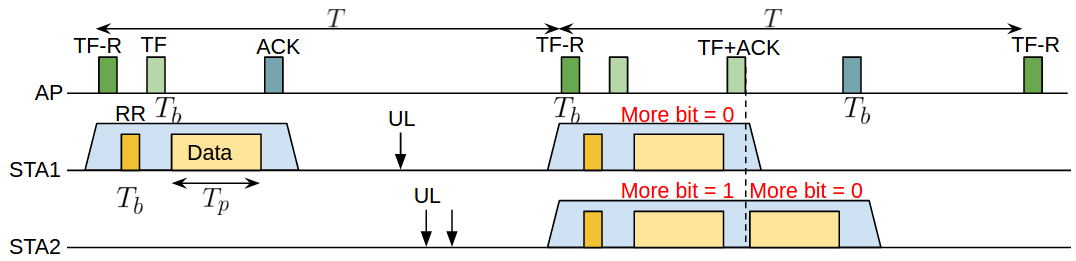
\includegraphics[scale=0.25]{./figure/ps_ax.png}
\label{fig_ps_ax_2}
\end{figure}
\end{frame}

% frame
\begin{frame}{Compute $UL$ and $R$}
	% column 
  \begin{columns}[T,onlytextwidth]
	% column 1    
    \column{0.4\textwidth}
	% equation
	\begin{align}
	%\begin{split}
	UL  &= \lambda T \sum_{k=0}^{\infty} (1-p_s)^k \nonumber\\ 
		&= \frac{\lambda T}{p_s} 
	%\end{split}
	\label{equ_UL}
	\end{align}
	
	% equation
	\begin{align}
	\label{equ_R}
	R   &= \frac{n_{ch}}{N_s}
	\end{align}

 % column 2
\column{0.5\textwidth}
% notation block
\metroset{block=fill}
\begin{alertblock}{Notations}
    $UL$: num. of UL packets to be sent in the current TF period given suc RR\\
    $R$: allocated resource  (date rate)\\
    $n_{ch}$: num. of channels\\
    $N_s$: num. of suc RR STA \\
    $p_s$: prob. of suc RR 
\end{alertblock}
\end{columns}
If UL packets are not transmitted in current TF period, it will be deferred to next TF period, as equation \ref{equ_UL}.\\
For resource allocation, resource is bandwidth that STA could use. Here, use channel number to represent it.  

\end{frame}

% frame
\begin{frame}{Compute $N_s$ ,$p_s$ and $p_{ss}$}
	% column 
  \begin{columns}[T,onlytextwidth]
	% column 1    
    \column{0.45\textwidth}
    % equation of N_s
	\begin{align}
	\label{equ_Ns}
	N_s &= \min\lbrace n_s, n_{ch}\rbrace \\
	% equation of p_s
	p_s &= p_{sc}p_{ss} \\
	p_{ss} &=
	\begin{cases}
	 \frac{n_{ch}}{n_s},  &n_s > n_{ch}\\
	 1, 				& 1 \leq n_s \leq n_{ch} \\
	 0, 				& n_s = 0
	\end{cases}	
	\label{equ_pss}
	\end{align}
	
	% column 2    
    \column{0.5\textwidth}
	% notation block
	\metroset{block=fill}
	\begin{alertblock}{Notations}
		$N_s$: num. of suc RR STAs \\
    		$n_s$: num. of suc contending STAs \\
    		$n_{ch}$: num. of channels\\
		$p_s$: prob. of suc RR \\
		$p_{sc}$: prob. of suc contending \\   
		$p_{ss}$: prob. of being selected 
	\end{alertblock}
	\end{columns}

Resource Request  (RR) are divided into two stages, one for random contending, another for AP selection. \\
If $n_s > n_{ch}$, which means not enough resource for request, AP will select $n_{ch}$ STAs. 
\end{frame}

% frame
\begin{frame}{Compute $p_{sc}$ and $n_{s}$}
	% column 
  \begin{columns}[T,onlytextwidth]
	% column 1    
    \column{0.45\textwidth}
	% equation
	\begin{align}
	n_c (t) = &n_c(t-1)- N_s(t-1) + \lambda^\prime,  \\
	\lambda^\prime \sim \mathrm{B} (&\mathbb{N,P}), \nonumber\\
	\mathbb{N} = n-&n_c(t-1)+N_s(t-1), \nonumber \\
	\mathbb{P} = 1-&e^{-\lambda T} \nonumber
	\end{align}
	
	% equation
	\begin{align}
		p_{sc} =  (\frac{c_w-1}{c_w})^{n_c (t)-1} 	
	\end{align}
	% column 2    
    \column{0.5\textwidth}
    % notation block
	\metroset{block=fill}
	\begin{alertblock}{Notations}
		$\lambda^\prime$: new arrival STAs for this TF-R period \\
		$n$: num. of all STAs \\
		$n_c$: num. of contending STA\\
    		$n_s$: num. of suc contending STAs \\
    		$n_{ch}$: num. of channels\\
    		$N_s$: num. of suc RR STAs \\
		$c_w$: contending window size\\
    		$p_{sc}$: prob. of suc contending    
	\end{alertblock}
    	\end{columns}
     
    	% equation
	\begin{align}
		P\lbrace n_s = k \rbrace  = \sum_{j=k}^{n_c}  (-1)^{k+j}\binom{j}{k}S_j, \; 1\leq k \leq \min\lbrace n_c,c_w \rbrace\\	
		S_j = \binom {c_w}{j} \prod_{i=1}^k \binom{n_c-i+1}{1}\frac{1}{c_w-i+1} (1-\frac{1}{c_w-i+1})^{n_c-i} \nonumber
	\end{align}	
	Above is the case when $n_c < c_w$. More derivation see appendix.
\end{frame}

% frame
\begin{frame}{Expected value}
% equation
\begin{align}
E[p_t] &= 1-e^{-\lambda T} \\
E[n_c] &= \lceil \frac{(1-e^{-\lambda T})n}{1-(1-p_s)e^{-\lambda T}}  \rceil \\
		&\approx \lceil (1-e^{-\lambda T})n \rceil\\
E[p_{sc}] &=  (\frac{c_w-1}{c_w})^{E[n_c]-1}
\end{align}

When traffic load is very light, $\lambda$ is small, we need take ceiling of $E[n_c]$ to avoid $E[p_{sc}]>1$.
This approach only reduces the power efficiency.
% equation 

\begin{align}
E[p_{ss}] &= \sum^{n_{ch}}_{k=1}P\lbrace n_s = k \rbrace 
	+  \sum_{k=n_{ch}+1}^{n_c}\frac{n_{ch}}{k}P\lbrace n_s = k \rbrace
\end{align}

Then probability of success RR is 
\begin{align}
E[p_{s}] = E[p_{sc}]E[p_{ss}]
\end{align}
\end{frame}

% frame
\begin{frame}{Expected value}
With distribution of $n_s$ and definition of $N_s$  (Equation \ref{equ_Ns}), we have 
\begin{align}
E[N_s] &= \sum_{k=1}^{n_{ch}}kP\lbrace n_s =k \rbrace  + P\lbrace n_s > n_{ch} \rbrace n_{ch}  
\end{align}

Then recall Equation \ref{equ_R} of $R$
\begin{align}
E[R] = n_{ch}/E[N_s]
\end{align}

Now, we have $\bigtriangleup_{TX}$ and $\bigtriangleup_{RX}$, see Equation \ref{equ_tx} and \ref{equ_rx}, so as to $\bigtriangleup_{idle}$ and $\bigtriangleup_{doze}$. 
At last substitute into Equation \ref{equ_energy} to obtain the energy consumption.
\end{frame}
\subsection{Numerical Result}
% frame
\begin{frame}{Numerical Results--System Setup}
	% column
\begin{columns}[T,onlytextwidth]
	% column 1    
	\column{0.5\textwidth}
	\justify
	The time scale is based on $\mu s$. $T_p$ is the duration for transmitting a packet under normalized data rate. \\
	Our model assumes a random access procedure with constant window size 32. It is a big assumption. \\
	For power consumption, I assume $P_{TX}$ is independent of the bandwidth. \\
	And I also ignore the inter-frame spacing (IFS) and contending procedure of TF. \\
	% column2
    \column{0.45\textwidth}
% table
 \begin{table}
    \caption{System Parameter Setting for Analysis}
    \begin{tabular}{l|l}
      %\toprule
	\hline
	$T_b$& 50 $\mu s$ \\
	$T_p$& 500 $\mu s$ \\
	$n_{ch}$& 10 \\
	$c_w$ &32 \\
	$P_{TX}$& 1000 $mW$ \\
	$P_{RX}$& 600 $mW$ \\
	$P_{idle}$& 300 $mW$ \\
	$P_{doze}$& 150 $mW$ \\
     % \midrule
     % \bottomrule
	\hline    
    \end{tabular}
  \end{table}
  \end{columns}
  	All above assumptions or simplifications are based on the first glimpse of the model and the system, 
	figuring out the key factors and unexpected problems of some mechanism.  
\end{frame}

% frame 
\begin{frame}{Numerical Results--Power Save Performance}
\begin{figure}
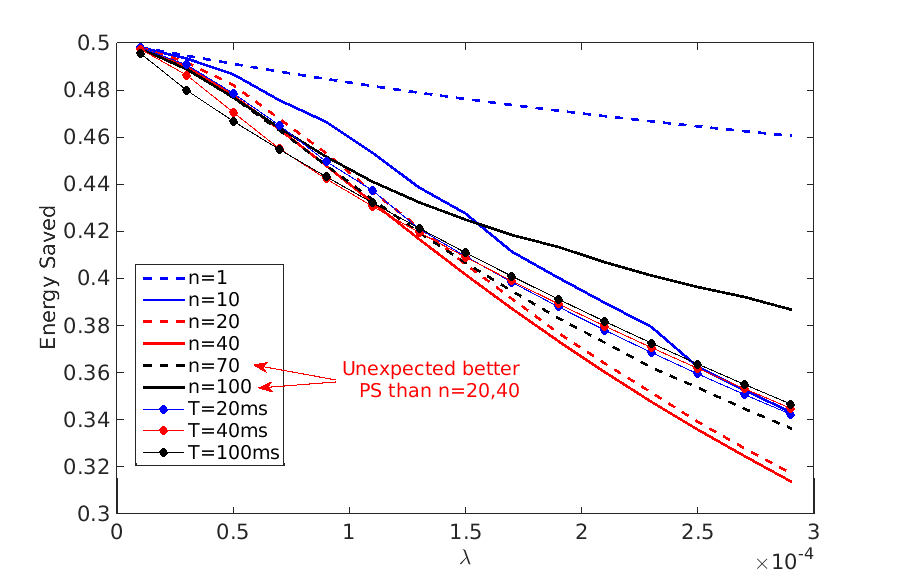
\includegraphics[scale=0.45]{./figure/test_per.png}
\caption{Power Save Performance with Different Parameters}
\label{test_per}
\end{figure}
\end{frame}

% frame
\begin{frame}{Numerical Results--Power Save Performance}
We find most results are as we thought. 
\begin{itemize}
\item
It's intuitive that as $\lambda$ increasing, energy efficiency reduces, because our the effective transmission increase, the remaining waste energy are less.
\item 
Period $T$ is not important for energy saving, but should affect latency a lot.
\item
Intuitively, as $n$ increases (more dense), PS will degrade. However, in our simulation, it's not always right. 
\end{itemize}
% figure
\begin{figure}
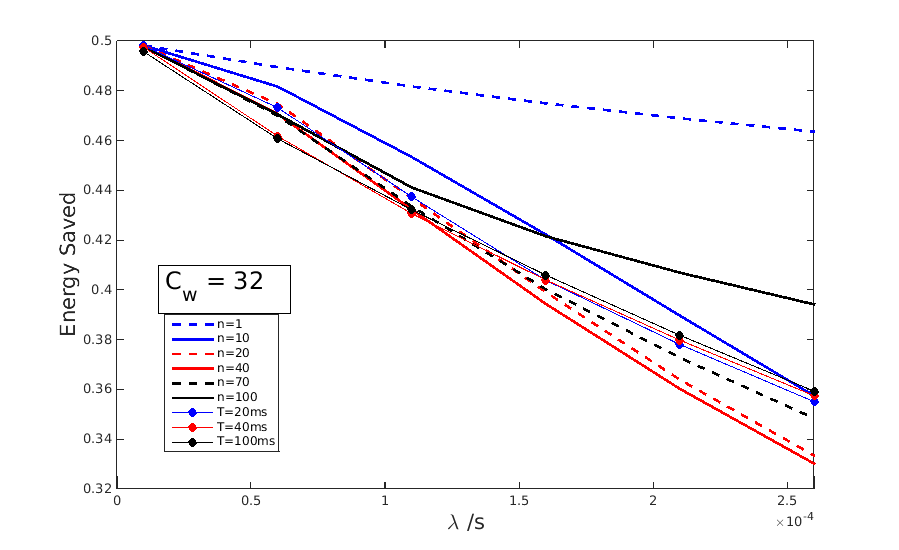
\includegraphics[scale=0.26]{./figure/test_per_2.png}
%\caption{Power Save Performance with Different Parameters}
%\label{test_per}
\end{figure}
\end{frame}

% frame
\begin{frame}{Numerical Results--$n_s$ behavior}
$n_{s1}$ is derivated using the distribution of $n_s$, and $n_{s2}$ is derivated using equation \ref{expt_ns}.
It validates the distribution of $n_s$.\\
Again, an unexpected phenomenon is as $n>35$, $n_s$ and $N_s$ both decrease. 
It is because contention window $c_w$ is small for more STAs.
% figure
\begin{figure}
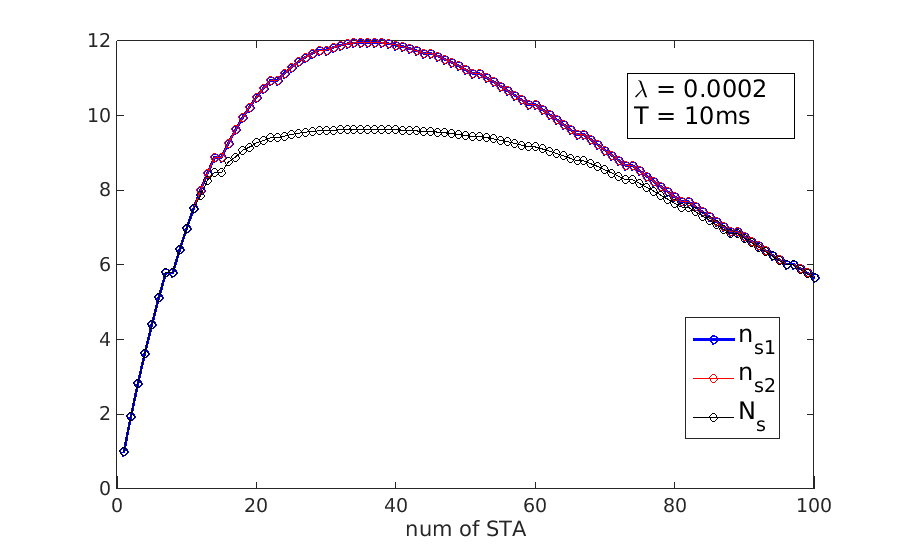
\includegraphics[scale=0.35]{./figure/test_ns.png}
\caption{Success Contending STAs and Success RR STAs}
\label{test_ns}
\end{figure}
\end{frame}

% frame
\begin{frame}{Numerical Results--$p_{sc}$, $p_{ss}$, $p_s$}
It is \textbf{expected} now that $p_{ss}$ will increase after $n=35$.
Recalling equation \ref{equ_pss}, since $N_s$ decrease after $n=35$, $p_{ss}$ increases. \\
Also, with $N_s$ decreasing, $R$ increase; with $p_s$ increasing, both above help \textbf{power save}. 
% figure
\begin{figure}
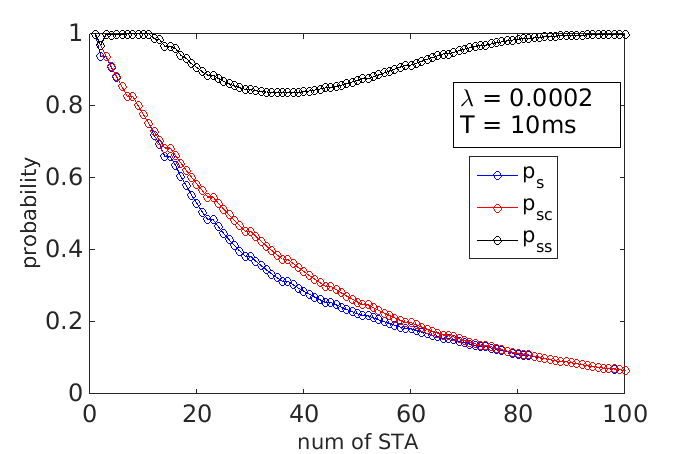
\includegraphics[scale=0.45]{./figure/test_ps.png}
\caption{Probability of Success Contending ($p_{sc}$), Selecting ($p_{ss}$) and RR ($p_{ps}$)}
\label{test_per}
\end{figure}
\end{frame}

% frame 
\begin{frame}{Numerical Results--PS with Modified $c_w$}
We can see that larger $c_w$ will make the result as we thought intuitively that the more STAs, the power save is more serious.
The unexpected phenomenon comes from our big assumption "random access for RR with constant $c_w=32$".
\begin{figure}
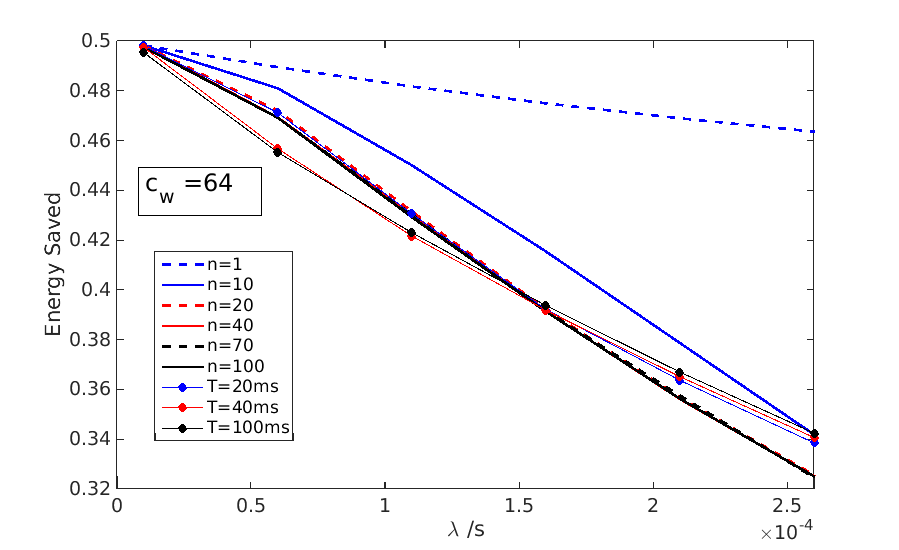
\includegraphics[scale=0.36]{./figure/test_per_3.png}
\caption{Power Save Performance with $c_w=64$}
\label{fig_PS_2}
\end{figure}
\end{frame}
\section{Issues}
% frame
\begin{frame}{Issues}
	What I did
	\begin{itemize}
		\item
		A power save design for 802.11ax UL. 
		\item 
		A model and numerical results help obtain the insight of the design.
		\item 
		A discrete-time event simulation.
	\end{itemize}
    In progress idea and work
    \begin{itemize}
        \item
        A improved model to do \alert{Latency Analysis} (queueing model)
        \item \alert{Dense Network}: 
        A scheduler to schedule UL/DL efficiently. The hardness is that UL traffic is unknown.
        \item 
        Learn how to predict UL traffic. Predict according to last TF period.
    \end{itemize}
    Think more\\
    \begin{itemize}
    \item
    What if unexpected interference?    
 %    Simulation with NS3
    \end{itemize}
\end{frame}

%
\section{Appendix}
% frame
\begin{frame}{Distribution of $n_s$}
	The number of successful contending STAs in random access equals to a problem as follows. \\
	Given \alert{$n$} buckets, and \alert{$m$} balls, put the balls randomly into the buckets. 
	We want to know the distribution of number of buckets which contain only one ball.
	Let \alert{$X$} be the number of such buckets. \alert{$Y_i$} denotes number of balls in bucket $i$. 
	Then
	\begin{align*}
	X = \sum_{i=1}^n\mathds{1}_{Y_i = 1} 
	\end{align*}
	\alert{$A_i$}: event that bucket $i$ contains only one ball. \\
	To begin, for $1\leq k \leq m$, let
	\begin{align*}
	S_k = \sum_{i_i< \ldots < i_k}P (A_{i_1}\ldots A_{i_k})
	\end{align*}
	equal the sum of the probabilities of all the $\binom{n}{k}$ intersections of $k$ distinct events. 
\end{frame}

% frame
\begin{frame}{Distribution of $n_s$}
	With above formulation, the distribution of $X$ is given as follows. \\ \cite[p.74-76]{ross2014introduction}
	\begin{align*}
		P\lbrace X = k \rbrace 
			&= \sum_{j=k}^n  (-1)^{k+j}\binom{j}{k}S_j \\ 
			&= S_k - \binom{k+1}{k}S_{k+1}+\cdots + (-1)^{n-k}\binom{n}{k}S_{n} 
	\end{align*}	
	\begin{align*}
		S_j = \binom {n}{j} \prod_{i=0}^{j-1} \binom{m-i}{1}\frac{1}{n-i} (1-\frac{1}{n-i})^{m-i-1} \nonumber
	\end{align*}
	
	The expected value is easy to compute.
	\begin{align}
	E[X] = E[\sum_{i=1}^n\mathds{1}_{Y_i = 1}] = \sum_{i=1}^nE[\mathds{1}_{Y_i = 1}] = \sum_{i=1}^n\binom{m}{1}\frac{1}{n} (1-\frac{1}{n})^{m-1}
	\label{expt_ns}
	\end{align}
\end{frame}

\begin{frame}[allowframebreaks]{References}
    \bibliography{demo}
    \bibliographystyle{abbrv}
\end{frame}

% frame    
\plain{Thanks}    
    
\end{document}
